\section{Block Ciphers}
\subsection{Overview}
\begin{frame}{Overview Block Ciphers}
	\begin{block}{Examples of Block Ciphers}
		\begin{itemize}
			\item DES (Feistel Network)
			\item AES (Substitution Permutation Network)
			\item \present{} (Lightweight Block Cipher)
		\end{itemize}
	\end{block}
\end{frame}

\subsection{Design Strategy}
\begin{frame}{DES}{Feistel Networks}
	\begin{columns}[onlytextwidth]
		\visible<1->{%
			\begin{column}{.50\textwidth}
				\begin{block}{DES}
					\begin{itemize}
						\item proposed 1975
						\item developed: IBM --- and NSA \Sey{}
					\end{itemize}
					\begin{itemize}
						\item 56 Bit Key
						\item 64 Bit Blocksize
					\end{itemize}
					\begin{itemize}
						\item 16 Rounds
						\item 8 S-boxes: $6 \rightarrow 4$ Bit
					\end{itemize}
				\end{block}
			\end{column}
		}
		\hfill
		\visible<2->{%
			\begin{column}{.41\textwidth}
				\begin{block}{Feistel Network}
					\centering
					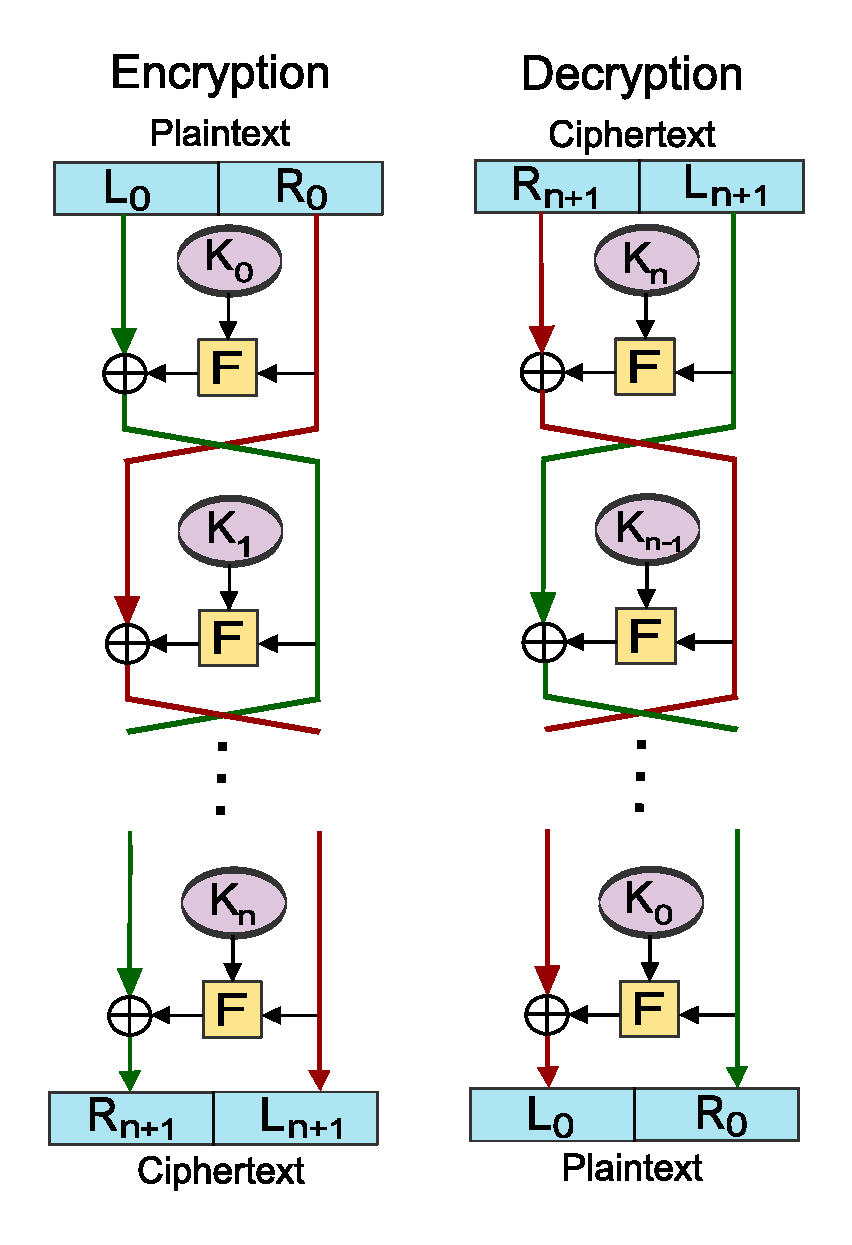
\includegraphics[height=.705\textheight]{data/wiki/Feistel}
				\end{block}
			\end{column}
		}
	\end{columns}
\end{frame}

\begin{frame}{AES}{Substitution Permutation Networks}
	\begin{columns}[onlytextwidth]
		\visible<1->{%
			\begin{column}{.50\textwidth}
				\begin{block}{AES}
					\begin{itemize}
						\item proposed 1998
						\item developed: Daemen and Rijmen
					\end{itemize}
					\begin{itemize}
						\item 128, 192, 256 Bit Key
						\item 128 Bit Blocksize
					\end{itemize}
					\begin{itemize}
						\item 10, 12, 14 Rounds
						\item 1 S-box: $8 \rightarrow 8$ Bits
					\end{itemize}
				\end{block}
			\end{column}
		}
		\hfill
		\visible<2->{%
			\begin{column}{.41\textwidth}
				\begin{block}{SPN}
					\centering
					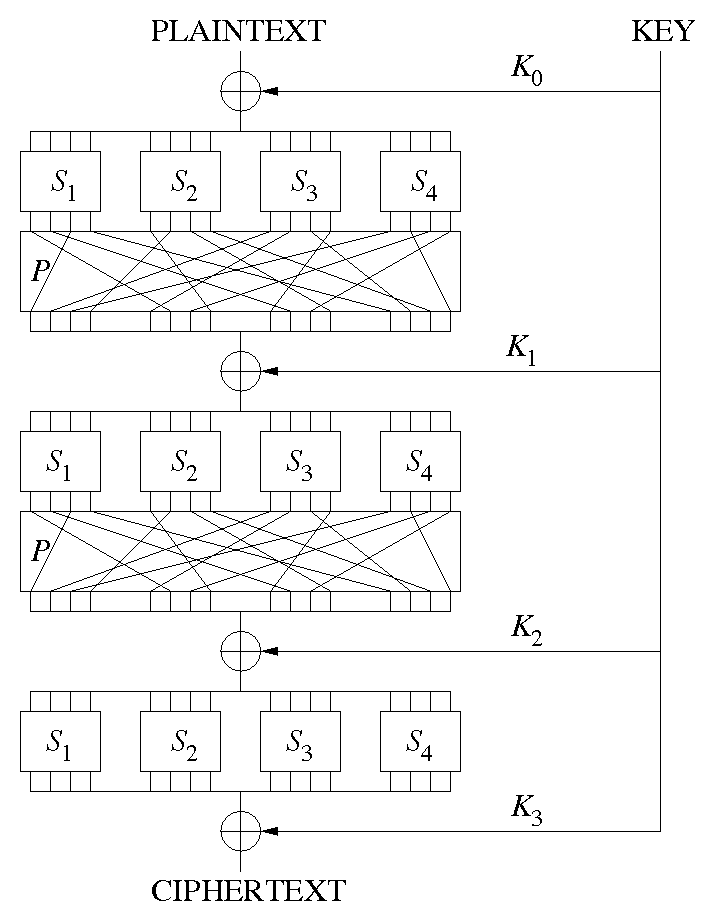
\includegraphics[height=.705\textheight]{data/wiki/SPN}
				\end{block}
			\end{column}
		}
	\end{columns}
\end{frame}

\begin{frame}{Design Strategy}
	\begin{columns}[T]
		\visible<1->{%
			\begin{column}{.48\textwidth}
				\begin{exampleblock}{The Mathematicians Approach}
					\begin{itemize}
						\item based on security proofs
						\item reduce breaking the cipher to mathematical hard problems
							\visible<2->{%
							\item slow \Annoey{}
							}
							\visible<3->{%
							\item fat \Sey{}
							}
							\visible<4->{%
							\item too much math \NiceReapey{}
							}
					\end{itemize}
				\end{exampleblock}
			\end{column}
		}
		\hfill
		\visible<5->{%
			\begin{column}{.48\textwidth}
				\begin{alertblock}{The Engineers Approach}
					\begin{itemize}
						\item build efficient scheme
						\item such that it is resistant against known attacks
							\visible<6->{%
							\item fast \Smiley{}
							}
							\visible<7->{%
							\item small \Laughey{}
							}
							\visible<8->{%
							\item few math \Ninja{}
							}
					\end{itemize}
				\end{alertblock}
			\end{column}
		}
	\end{columns}
\end{frame}

\subsection{Lightweight Crypto}
\begin{frame}{Lightweight Crypto}{Buzzword Alarm!}
	\visible<1->{%
	\begin{block}{Ubiquitous Computing}
		\begin{itemize}
			\item very constrained devices needed for Internet of Things
			\item need crypto schemes with very low requirements
		\end{itemize}
	\end{block}
}

	\vspace{5mm}

	\visible<2->{%
	\begin{center}
		How efficient \emph{(small, fast, low power, low latency)}

		can we be, without sacrificing security?
	\end{center}
}
\end{frame}

\begin{frame}{\present{}}
\visible<1->{%
	\begin{block}{\present{}}
		\begin{columns}[onlytextwidth]
			\begin{column}{.59\textwidth}
				\begin{itemize}
					\item proposed 2007
					\item developed: Orange Labs, RUB, DTU
					\item 1 S-box: $4 \rightarrow 4$ Bits
				\end{itemize}
			\end{column}
			\begin{column}{.41\textwidth}
				\begin{itemize}
					\item 80, 128 Bit Key
					\item 64 Bit Blocksize
					\item 31 Rounds
				\end{itemize}
			\end{column}
		\end{columns}
		\vspace{3mm}
	\end{block}
}

\visible<2->{%
	\begin{itemize}
		\item Let $F_{k_i} : \mathbb{F}_2^{64} \rightarrow \mathbb{F}_2^{64}$ be
			\present{}'s round function:
	\end{itemize}
}

\visible<3->{%
	\begin{block}{\present{} Round}
		\begin{figure}[!ht]
			\centering
			\begin{tikzpicture}[%
					x={(0.04\textwidth,0)},
					y={(0,0.03\textwidth)}
				]

				\def \maxround{2}
				\def \roundH{5}
				\def \round{1}

				\def \TEST{\roundH*\maxround-\roundH*\round+0.5}
				\def \BEST{\roundH*\maxround-\roundH*\round-\roundH+2.5}
				%Sboxes with input and output lines and xor for the key
				\foreach \i in {0,1,2,3,4,5,6,7,8,9,10,11,12,13,14,15}{%
					%Input and output lines
					\foreach \j in {1,2,3,4}{%
						%output lines
						\draw[color=saphierblau] (1.5*\i+0.2*\j,\roundH*\maxround-\roundH*\round+1) -- (1.5*\i+0.2*\j,\roundH*\maxround-\roundH*\round+0.5);

						%input lines
						\draw[color=saphierblau] (1.5*\i+0.2*\j,\roundH*\maxround-\roundH*\round+2) -- (1.5*\i+0.2*\j,\roundH*\maxround-\roundH*\round+2.5);

						%XOR
						\draw[color=saphierblau] (1.5*\i+0.2*\j,\roundH*\maxround-\roundH*\round+2.25) circle (0.1);
						\draw[color=saphierblau] (1.5*\i+0.2*\j-0.1,\roundH*\maxround-\roundH*\round+2.25) -- (1.5*\i+0.2*\j+0.1,\roundH*\maxround-\roundH*\round+2.25);
					}

					%Sbox
					\draw[color=saphierblau] (1.5*\i,\roundH*\maxround-\roundH*\round+1) rectangle (1.5*\i+1,\roundH*\maxround-\roundH*\round+2);
					\node[color=saphierblau] at (1.5*\i+0.5,\roundH*\maxround-\roundH*\round+1.5) {S};
				}

				%The P-layer
				\draw[color=saphierblau] ( 0.2,\TEST) -- ( 0.2,\BEST); \draw[color=saphierblau] ( 0.4,\TEST) -- ( 6.2,\BEST);
				\draw[color=saphierblau] ( 0.6,\TEST) -- (12.2,\BEST); \draw[color=saphierblau] ( 0.8,\TEST) -- (18.2,\BEST);
				\draw[color=saphierblau] ( 1.7,\TEST) -- ( 0.4,\BEST); \draw[color=saphierblau] ( 1.9,\TEST) -- ( 6.4,\BEST);
				\draw[color=saphierblau] ( 2.1,\TEST) -- (12.4,\BEST); \draw[color=saphierblau] ( 2.3,\TEST) -- (18.4,\BEST);
				\draw[color=saphierblau] ( 3.2,\TEST) -- ( 0.6,\BEST); \draw[color=saphierblau] ( 3.4,\TEST) -- ( 6.6,\BEST);
				\draw[color=saphierblau] ( 3.6,\TEST) -- (12.6,\BEST); \draw[color=saphierblau] ( 3.8,\TEST) -- (18.6,\BEST);
				\draw[color=saphierblau] ( 4.7,\TEST) -- ( 0.8,\BEST); \draw[color=saphierblau] ( 4.9,\TEST) -- ( 6.8,\BEST);
				\draw[color=saphierblau] ( 5.1,\TEST) -- (12.8,\BEST); \draw[color=saphierblau] ( 5.3,\TEST) -- (18.8,\BEST);
				\draw[color=saphierblau] ( 6.2,\TEST) -- ( 1.7,\BEST); \draw[color=saphierblau] ( 6.4,\TEST) -- ( 7.7,\BEST);
				\draw[color=saphierblau] ( 6.6,\TEST) -- (13.7,\BEST); \draw[color=saphierblau] ( 6.8,\TEST) -- (19.7,\BEST);
				\draw[color=saphierblau] ( 7.7,\TEST) -- ( 1.9,\BEST); \draw[color=saphierblau] ( 7.9,\TEST) -- ( 7.9,\BEST);
				\draw[color=saphierblau] ( 8.1,\TEST) -- (13.9,\BEST); \draw[color=saphierblau] ( 8.3,\TEST) -- (19.9,\BEST);
				\draw[color=saphierblau] ( 9.2,\TEST) -- ( 2.1,\BEST); \draw[color=saphierblau] ( 9.4,\TEST) -- ( 8.1,\BEST);
				\draw[color=saphierblau] ( 9.6,\TEST) -- (14.1,\BEST); \draw[color=saphierblau] ( 9.8,\TEST) -- (20.1,\BEST);
				\draw[color=saphierblau] (10.7,\TEST) -- ( 2.3,\BEST); \draw[color=saphierblau] (10.9,\TEST) -- ( 8.3,\BEST);
				\draw[color=saphierblau] (11.1,\TEST) -- (14.3,\BEST); \draw[color=saphierblau] (11.3,\TEST) -- (20.3,\BEST);
				\draw[color=saphierblau] (12.2,\TEST) -- ( 3.2,\BEST); \draw[color=saphierblau] (12.4,\TEST) -- ( 9.2,\BEST);
				\draw[color=saphierblau] (12.6,\TEST) -- (15.2,\BEST); \draw[color=saphierblau] (12.8,\TEST) -- (21.2,\BEST);
				\draw[color=saphierblau] (13.7,\TEST) -- ( 3.4,\BEST); \draw[color=saphierblau] (13.9,\TEST) -- ( 9.4,\BEST);
				\draw[color=saphierblau] (14.1,\TEST) -- (15.4,\BEST); \draw[color=saphierblau] (14.3,\TEST) -- (21.4,\BEST);
				\draw[color=saphierblau] (15.2,\TEST) -- ( 3.6,\BEST); \draw[color=saphierblau] (15.4,\TEST) -- ( 9.6,\BEST);
				\draw[color=saphierblau] (15.6,\TEST) -- (15.6,\BEST); \draw[color=saphierblau] (15.8,\TEST) -- (21.6,\BEST);
				\draw[color=saphierblau] (16.7,\TEST) -- ( 3.8,\BEST); \draw[color=saphierblau] (16.9,\TEST) -- ( 9.8,\BEST);
				\draw[color=saphierblau] (17.1,\TEST) -- (15.8,\BEST); \draw[color=saphierblau] (17.3,\TEST) -- (21.8,\BEST);
				\draw[color=saphierblau] (18.2,\TEST) -- ( 4.7,\BEST); \draw[color=saphierblau] (18.4,\TEST) -- (10.7,\BEST);
				\draw[color=saphierblau] (18.6,\TEST) -- (16.7,\BEST); \draw[color=saphierblau] (18.8,\TEST) -- (22.7,\BEST);
				\draw[color=saphierblau] (19.7,\TEST) -- ( 4.9,\BEST); \draw[color=saphierblau] (19.9,\TEST) -- (10.9,\BEST);
				\draw[color=saphierblau] (20.1,\TEST) -- (16.9,\BEST); \draw[color=saphierblau] (20.3,\TEST) -- (22.9,\BEST);
				\draw[color=saphierblau] (21.2,\TEST) -- ( 5.1,\BEST); \draw[color=saphierblau] (21.4,\TEST) -- (11.1,\BEST);
				\draw[color=saphierblau] (21.6,\TEST) -- (17.1,\BEST); \draw[color=saphierblau] (21.8,\TEST) -- (23.1,\BEST);
				\draw[color=saphierblau] (22.7,\TEST) -- ( 5.3,\BEST); \draw[color=saphierblau] (22.9,\TEST) -- (11.3,\BEST);
				\draw[color=saphierblau] (23.1,\TEST) -- (17.3,\BEST); \draw[color=saphierblau] (23.3,\TEST) -- (23.3,\BEST);

			\end{tikzpicture}
		\end{figure}
	\end{block}
}

\end{frame}

\section{Linear Cryptanalysis}
\subsection{Overview}
\begin{frame}{Overview Attacks}
	\begin{columns}[onlytextwidth]
		\begin{column}{.58\textwidth}
	\begin{block}{Attacks on Block Ciphers}
		\begin{itemize}
			\item Differential Cryptanalysis
			\item \emph{Linear Cryptanalysis}
		\end{itemize}
		\begin{itemize}
			\item Integral,
			\item Interpolation,
			\item Statistical Saturation,
			\item Invariant Subspace,
			\item Algebraic,
			\item Related Key,
			\item \ldots
		\end{itemize}
	\end{block}
		\end{column}
		\hfill
		\begin{column}{.38\textwidth}
			\begin{figure}[!ht]
				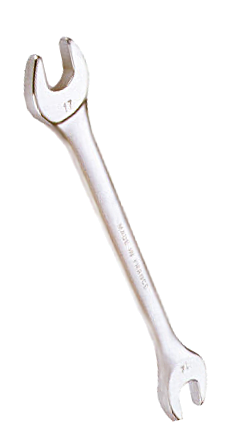
\includegraphics[height=50mm]{data/wiki/wrench}
			\end{figure}
		\end{column}
	\end{columns}
\end{frame}

\subsection{Linear Cryptanalysis}
\begin{frame}{Introduction to Linear Cryptanalysis}
	\begin{columns}[T]
		\begin{column}{.58\textwidth}
			\begin{itemize}
				\item invented by Matsui 1993--1994
				\item broke DES
				\item together with Differential Cryptanalysis
						most used attack on block ciphers
			\end{itemize}
		\end{column}
		\hfill
		\begin{column}{.38\textwidth}
			\begin{figure}[!ht]
				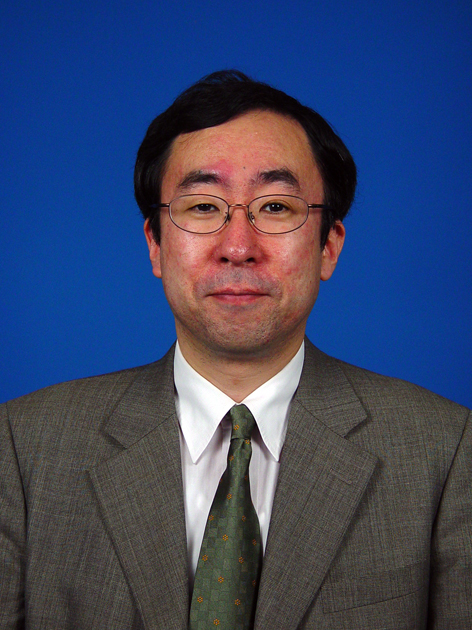
\includegraphics[height=50mm]{data/matsui.jpg}
			\end{figure}
		\end{column}
	\end{columns}\blfootnote{\scriptsize Image: \url{http://www.isce2009.ryukoku.ac.jp/eng/keynote_address.html}}
\end{frame}

\begin{frame}{Basic Idea: Linear Approximations}{Dot-Product, Masks and Linear Bias}
	\vspace{-10pt}
	\visible<1->{%
	\begin{itemize}
		\item Can we linear approximate a function $F : \mathbb{F}_2^n \rightarrow \mathbb{F}_2^n$?
	\end{itemize}
	}

	\vspace{-10pt}
	\begin{columns}[T]
	\visible<2->{%
		\begin{column}{0.48\textwidth}
			\begin{block}{Dot-Product}
				\begin{equation*}
				\vspace{-2pt}
					\langle \alpha, x \rangle = \bigoplus_{i=0}^{n-1} \alpha_i x_i
				\end{equation*}
			\end{block}
		\end{column}
	}

	\visible<3->{%
		\begin{column}{0.48\textwidth}
			\begin{block}{Mask}
				Let $\alpha, \beta, x \in \mathbb{F}_2^n$ and
				%\vspace{-6pt}
				\begin{equation}
					\langle \alpha, x \rangle = \langle \beta, F(x) \rangle \label{equ:masks}
				\end{equation}
			\end{block}
		\end{column}
	}
	\end{columns}
	\visible<3->{%
	\begin{itemize}
		\item We say $\alpha$ is an \emph{input mask} and $\beta$ is an \emph{output mask}.
		\item Eq.~\ref{equ:masks} does not hold for every input/output masks.
	\end{itemize}
	}

	\visible<4->{%
	\begin{itemize}
		\item It is \emph{biased}, i.e., $\text{Pr}[\langle \alpha, x \rangle = \langle
			\beta, F(x) \rangle] = \frac{1}{2} - \epsilon(\alpha, \beta)$.
	\end{itemize}
	}
\end{frame}

\begin{frame}{Example}{Masks for 2-Round reduced \present{}}
	\begin{block}{Mask $(21, 21)$ over 2 rounds}
		\begin{figure}[!ht]
			\centering
			\begin{tikzpicture}[%
					x={(0.04\textwidth,0)},
					y={(0,0.03\textwidth)}
				]

				\def \maxround{2}
				\def \roundH{5}

				\foreach \round in {1,2}{%
					\def \TEST{\roundH*\maxround-\roundH*\round+0.5}
					\def \BEST{\roundH*\maxround-\roundH*\round-\roundH+2.5}
					%Sboxes with input and output lines and xor for the key
					\foreach \i in {0,1,2,3,4,5,6,7,8,9,10,11,12,13,14,15}{%Sbox
						\draw[color=saphierblau] (1.5*\i,\roundH*\maxround-\roundH*\round+1)
							rectangle (1.5*\i+1,\roundH*\maxround-\roundH*\round+2);
						\node[color=saphierblau] at (1.5*\i+0.5,\roundH*\maxround-\roundH*\round+1.5) {S};

						%Input and output lines
						\foreach \j in {1,2,3,4}{%output lines
							\draw[color=saphierblau] (1.5*\i+0.2*\j,\roundH*\maxround-\roundH*\round+1) -- (1.5*\i+0.2*\j,\roundH*\maxround-\roundH*\round+0.5);

							%input lines
							\draw[color=saphierblau] (1.5*\i+0.2*\j,\roundH*\maxround-\roundH*\round+2) -- (1.5*\i+0.2*\j,\roundH*\maxround-\roundH*\round+2.5);

							%XOR
							\draw[color=saphierblau] (1.5*\i+0.2*\j,\roundH*\maxround-\roundH*\round+2.25) circle (0.1);
							\draw[color=saphierblau] (1.5*\i+0.2*\j-0.1,\roundH*\maxround-\roundH*\round+2.25) -- (1.5*\i+0.2*\j+0.1,\roundH*\maxround-\roundH*\round+2.25);
						}
					}

					%The P-layer
					\DrawPresentPLayer{\TEST}{\BEST}
				}

				\def \round{3}
				%Input lines and xor for the key
				\foreach \i in {0,1,2,3,4,5,6,7,8,9,10,11,12,13,14,15}{%Input lines
					\foreach \j in {1,2,3,4}{%input lines
						\draw[color=saphierblau] (1.5*\i+0.2*\j,\roundH*\maxround-\roundH*\round+2) -- (1.5*\i+0.2*\j,\roundH*\maxround-\roundH*\round+2.5);

						%XOR
						\draw[color=saphierblau] (1.5*\i+0.2*\j,\roundH*\maxround-\roundH*\round+2.25) circle (0.1);
						\draw[color=saphierblau] (1.5*\i+0.2*\j-0.1,\roundH*\maxround-\roundH*\round+2.25) -- (1.5*\i+0.2*\j+0.1,\roundH*\maxround-\roundH*\round+2.25);
					}
				}

				% highlight a path
				\def\ia{10}
				\def\ib{10}
				\def\ic{10}
				\def\id{10}
				\def\ie{10}

				\def\ja{3}
				\def\jb{3}
				\def\jc{3}
				\def\jd{3}
				\def\je{3}

				%input lines
				\draw[color=red, very thick]
					(1.5*\ia+0.2*\ja,\roundH*\maxround-\roundH*1+2) --
					(1.5*\ia+0.2*\ja,\roundH*\maxround-\roundH*1+2.5);
				%output lines
				\draw[color=red, very thick]
					(1.5*\ib+0.2*\jb,\roundH*\maxround-\roundH*1+1) --
					(1.5*\ib+0.2*\jb,\roundH*\maxround-\roundH*1+0.5);
				%XOR
				\draw[color=red, very thick]
					(1.5*\ia+0.2*\ja,\roundH*\maxround-\roundH*1+2.25) circle (0.1);
				\draw[color=red, very thick]
					(1.5*\ia+0.2*\ja-0.1,\roundH*\maxround-\roundH*1+2.25) --
					(1.5*\ia+0.2*\ja+0.1,\roundH*\maxround-\roundH*1+2.25);
				%P-layer
				\draw[color=red, very thick] (15.6,\roundH*\maxround-\roundH*1+0.5)
					--(15.6,\roundH*\maxround-\roundH*1-\roundH+2.5);

				%input lines
				\draw[color=red, very thick]
					(1.5*\ic+0.2*\jc,\roundH*\maxround-\roundH*2+2) --
					(1.5*\ic+0.2*\jc,\roundH*\maxround-\roundH*2+2.5);
				%output lines
				\draw[color=red, very thick]
					(1.5*\id+0.2*\jd,\roundH*\maxround-\roundH*2+1) --
					(1.5*\id+0.2*\jd,\roundH*\maxround-\roundH*2+0.5);
				%XOR
				\draw[color=red, very thick]
					(1.5*\ic+0.2*\jc,\roundH*\maxround-\roundH*2+2.25) circle (0.1);
				\draw[color=red, very thick]
					(1.5*\ic+0.2*\jc-0.1,\roundH*\maxround-\roundH*2+2.25) --
					(1.5*\ic+0.2*\jc+0.1,\roundH*\maxround-\roundH*2+2.25);
				%P-layer
				\draw[color=red, very thick] (15.6,\roundH*\maxround-\roundH*2+0.5)
					--(15.6,\roundH*\maxround-\roundH*2-\roundH+2.5);

				%input lines
				\draw[color=red, very thick]
					(1.5*\ie+0.2*\je,\roundH*\maxround-\roundH*3+2) --
					(1.5*\ie+0.2*\je,\roundH*\maxround-\roundH*3+2.5);
				%XOR
				\draw[color=red, very thick]
					(1.5*\ie+0.2*\je,\roundH*\maxround-\roundH*3+2.25) circle (0.1);
				\draw[color=red, very thick]
					(1.5*\ie+0.2*\je-0.1,\roundH*\maxround-\roundH*3+2.25) --
					(1.5*\ie+0.2*\je+0.1,\roundH*\maxround-\roundH*3+2.25);

			\end{tikzpicture}
		\end{figure}
	\end{block}
\end{frame}

\begin{frame}{Attack}
	\begin{columns}[T]
		\begin{column}{0.725\textwidth}
			\begin{block}{Approach}
				\visible<1->{%
					\begin{itemize}
						\item Find good approximation for all but last round
						\item that is: a good \emph{mask} over $r-1$ rounds
					\end{itemize}
				}
				\visible<2->{%
					\begin{itemize}
						\item With many plaintext/ciphertext pairs, we can observe
							the masks statistical behaviour
						\item that is: we can compute its \emph{bias}
					\end{itemize}
				}
				\visible<3->{%
					\begin{itemize}
						\item Hypothesis of Wrong Key Randomization
						\item Guess last round key and compute experimental bias
					\end{itemize}
				}
			\end{block}
		\end{column}
		\visible<3->{%
			\begin{column}{0.175\textwidth}
				\begin{block}{Hypothesis}
					\centering
					\begin{figure}[!ht]
						\begin{tikzpicture}[%
								scale=0.6,
								transform shape
							]
							\tikzset{line/.style={%
									draw,
									-latex',
									shorten <=1bp,
								shorten >=1bp}
							}
							\node (initial) {Plaintext};
							\node (preXOR) [XOR, below of=initial] {};
							\node (preKey) [right of=preXOR] {$k_0$};
							\node (fstSbox) [sbox, below of=preXOR] {S};
							\path [line] (initial) edge (preXOR);
							\path [line] (preKey) edge (preXOR);
							\path [line] (preXOR) edge (fstSbox);

							\node (fstXOR) [XOR, below of=fstSbox] {};
							\node (fstKey) [right of=fstXOR] {$k_1$};
							\node (sndSbox) [sbox, below of=fstXOR] {S};
							\path [line] (fstSbox) edge (fstXOR);
							\path [line] (fstKey) edge (fstXOR);
							\path [line] (fstXOR) edge (sndSbox);

							\node (sndXOR) [XOR, below of=sndSbox] {};
							\node (sndKey) [right of=sndXOR] {$k_2$};
							\node (trdSbox) [sbox, below of=sndXOR] {S};
							\path [line] (sndSbox) edge (sndXOR);
							\path [line] (sndKey) edge (sndXOR);
							\path [line] (sndXOR) edge (trdSbox);

							\node (postXOR) [XOR, below of=trdSbox] {};
							\node (postKey) [right of=postXOR] {$k_3$};
							\node (final) [below of=postXOR] {Ciphertext};
							\path [line] (trdSbox) edge (postXOR);
							\path [line] (postKey) edge (postXOR);
							\path [line] (postXOR) edge (final);
						\end{tikzpicture}
					\end{figure}
				\end{block}
			\end{column}
		}
	\end{columns}
\end{frame}

\begin{frame}{Example}{Linear Cryptanalysis of 3-Round reduced \present{}}
	\begin{block}{Attacking 3-Round reduced \present{}}
		\begin{figure}[!ht]
			\centering
			\begin{tikzpicture}[%
					x={(0.04\textwidth,0)},
					y={(0,0.03\textwidth)}
				]
				\def \maxround{3}
				\def \roundH{5}

				\foreach \round in {1,2}{%
					\def \TEST{\roundH*\maxround-\roundH*\round+0.5}
					\def \BEST{\roundH*\maxround-\roundH*\round-\roundH+2.5}
					%Sboxes with input and output lines and xor for the key
					\foreach \i in {0,1,2,3,4,5,6,7,8,9,10,11,12,13,14,15}{%Sbox
						\draw[color=saphierblau] (1.5*\i,\roundH*\maxround-\roundH*\round+1)
							rectangle (1.5*\i+1,\roundH*\maxround-\roundH*\round+2);
						\node[color=saphierblau] at (1.5*\i+0.5,\roundH*\maxround-\roundH*\round+1.5) {S};

						%Input and output lines
						\foreach \j in {1,2,3,4}{%output lines
							\draw[color=saphierblau] (1.5*\i+0.2*\j,\roundH*\maxround-\roundH*\round+1) -- (1.5*\i+0.2*\j,\roundH*\maxround-\roundH*\round+0.5);

							%input lines
							\draw[color=saphierblau] (1.5*\i+0.2*\j,\roundH*\maxround-\roundH*\round+2) -- (1.5*\i+0.2*\j,\roundH*\maxround-\roundH*\round+2.5);

							%XOR
							\draw[color=saphierblau] (1.5*\i+0.2*\j,\roundH*\maxround-\roundH*\round+2.25) circle (0.1);
							\draw[color=saphierblau] (1.5*\i+0.2*\j-0.1,\roundH*\maxround-\roundH*\round+2.25) -- (1.5*\i+0.2*\j+0.1,\roundH*\maxround-\roundH*\round+2.25);
						}
					}

					%The P-layer
					\DrawPresentPLayer{\TEST}{\BEST}
				}

				\def \round{3}
				%Sboxes with input and output lines and xor for the key
				\foreach \i in {0,1,2,3,4,5,6,7,8,9,10,11,12,13,14,15}{%Sbox
					\draw[color=saphierblau] (1.5*\i,\roundH*\maxround-\roundH*\round+1) rectangle (1.5*\i+1,\roundH*\maxround-\roundH*\round+2);
					\node[color=saphierblau] at (1.5*\i+0.5,\roundH*\maxround-\roundH*\round+1.5) {S};

					%Input and output lines
					\foreach \j in {1,2,3,4}{%output lines
						\draw[color=saphierblau] (1.5*\i+0.2*\j,\roundH*\maxround-\roundH*\round+1) -- (1.5*\i+0.2*\j,\roundH*\maxround-\roundH*\round+0.5);

						%input lines
						\draw[color=saphierblau] (1.5*\i+0.2*\j,\roundH*\maxround-\roundH*\round+2) -- (1.5*\i+0.2*\j,\roundH*\maxround-\roundH*\round+2.5);

						%XOR
						\draw[color=saphierblau] (1.5*\i+0.2*\j,\roundH*\maxround-\roundH*\round+2.25) circle (0.1);
						\draw[color=saphierblau] (1.5*\i+0.2*\j-0.1,\roundH*\maxround-\roundH*\round+2.25) -- (1.5*\i+0.2*\j+0.1,\roundH*\maxround-\roundH*\round+2.25);
					}
				}
				%post XOR
				\foreach \i in {0,1,2,3,4,5,6,7,8,9,11,12,13,14,15}{%
					\foreach \j in {1,2,3,4}{%
						\draw[color=saphierblau] (1.5*\i+0.2*\j,\roundH*\maxround-\roundH*\round+0.75) circle (0.1);
						\draw[color=saphierblau] (1.5*\i+0.2*\j-0.1,\roundH*\maxround-\roundH*\round+0.75) -- (1.5*\i+0.2*\j+0.1,\roundH*\maxround-\roundH*\round+0.75);
					}
				}
				\def \i{10}
				\foreach \j in {1,2,3,4}{%
					\draw[color=green] (1.5*\i+0.2*\j,\roundH*\maxround-\roundH*\round+1) -- (1.5*\i+0.2*\j,\roundH*\maxround-\roundH*\round+0.5);
					\draw[color=green] (1.5*\i+0.2*\j,\roundH*\maxround-\roundH*\round+0.75) circle (0.1);
					\draw[color=green] (1.5*\i+0.2*\j-0.1,\roundH*\maxround-\roundH*\round+0.75) -- (1.5*\i+0.2*\j+0.1,\roundH*\maxround-\roundH*\round+0.75);
				}

				% highlight a path
				\def\ia{10}
				\def\ib{10}
				\def\ic{10}
				\def\id{10}
				\def\ie{10}

				\def\ja{3}
				\def\jb{3}
				\def\jc{3}
				\def\jd{3}
				\def\je{3}

				%input lines
				\draw[color=red, very thick]
					(1.5*\ia+0.2*\ja,\roundH*\maxround-\roundH*1+2) --
					(1.5*\ia+0.2*\ja,\roundH*\maxround-\roundH*1+2.5);
				%output lines
				\draw[color=red, very thick]
					(1.5*\ib+0.2*\jb,\roundH*\maxround-\roundH*1+1) --
					(1.5*\ib+0.2*\jb,\roundH*\maxround-\roundH*1+0.5);
				%XOR
				\draw[color=red, very thick]
					(1.5*\ia+0.2*\ja,\roundH*\maxround-\roundH*1+2.25) circle (0.1);
				\draw[color=red, very thick]
					(1.5*\ia+0.2*\ja-0.1,\roundH*\maxround-\roundH*1+2.25) --
					(1.5*\ia+0.2*\ja+0.1,\roundH*\maxround-\roundH*1+2.25);
				%P-layer
				\draw[color=red, very thick] (15.6,\roundH*\maxround-\roundH*1+0.5)
					--(15.6,\roundH*\maxround-\roundH*1-\roundH+2.5);

				%input lines
				\draw[color=red, very thick]
					(1.5*\ic+0.2*\jc,\roundH*\maxround-\roundH*2+2) --
					(1.5*\ic+0.2*\jc,\roundH*\maxround-\roundH*2+2.5);
				%output lines
				\draw[color=red, very thick]
					(1.5*\id+0.2*\jd,\roundH*\maxround-\roundH*2+1) --
					(1.5*\id+0.2*\jd,\roundH*\maxround-\roundH*2+0.5);
				%XOR
				\draw[color=red, very thick]
					(1.5*\ic+0.2*\jc,\roundH*\maxround-\roundH*2+2.25) circle (0.1);
				\draw[color=red, very thick]
					(1.5*\ic+0.2*\jc-0.1,\roundH*\maxround-\roundH*2+2.25) --
					(1.5*\ic+0.2*\jc+0.1,\roundH*\maxround-\roundH*2+2.25);
				%P-layer
				\draw[color=red, very thick] (15.6,\roundH*\maxround-\roundH*2+0.5)
					--(15.6,\roundH*\maxround-\roundH*2-\roundH+2.5);

				%input lines
				\draw[color=red, very thick]
					(1.5*\ie+0.2*\je,\roundH*\maxround-\roundH*3+2) --
					(1.5*\ie+0.2*\je,\roundH*\maxround-\roundH*3+2.5);
				%XOR
				\draw[color=red, very thick]
					(1.5*\ie+0.2*\je,\roundH*\maxround-\roundH*3+2.25) circle (0.1);
				\draw[color=red, very thick]
					(1.5*\ie+0.2*\je-0.1,\roundH*\maxround-\roundH*3+2.25) --
					(1.5*\ie+0.2*\je+0.1,\roundH*\maxround-\roundH*3+2.25);

			\end{tikzpicture}
		\end{figure}
	\end{block}
\end{frame}

\subsection{Connection to Key Schedule}
\begin{frame}{Distributions}
	\visible<1->{%
	\begin{itemize}
		\item Attack complexity of linear cryptanalysis is proportional to $\frac{1}{\epsilon^2}$.
		\item In experiments, we observe a key dependency of the linear bias.
	\end{itemize}
	}
	\visible<2->{%
	\begin{itemize}
		\item The distribution of linear biases follows a normal distribution.
		\item Its width is defined by the variance.
	\end{itemize}
	}
	\visible<3->{%
	\begin{itemize}
		\item What happens with different key-schedules?
	\end{itemize}
	}
\end{frame}

\begin{frame}{Distributions}{Independent Round Keys}
	\begin{figure}
		\centering
		\begin{tikzpicture}
			\begin{axis}[
					every axis/.append style={font=\small},
					scaled ticks=false,
					no markers,
					xmin=-0.0002,
					ymin=0,
					ymax=475,
					xmax=0.0002,
					xlabel={Linear Correlation},
					height=7cm,
					width=11cm,
					ytick=\empty,
					xticklabels={-0.0002, -0.0001, 0, 0.0001, 0.0002},
					xtick={-0.0002, -0.0001, 0, 0.0001, 0.0002},
				]
				\addplot+[color=saphierblau, ybar, bar width=1pt, fill=saphierblau] table [x, y, col sep=space] {data/histo_indp.dat};
				\addplot+[color=red] table {data/gauss_est.dat};
				\draw[color=black, thin, dashed] (axis cs:-0.00005,\pgfkeysvalueof{/pgfplots/ymin}) -- (axis cs:-0.00005,\pgfkeysvalueof{/pgfplots/ymax});
				\draw[color=black, thin, dashed] (axis cs:0.00005,\pgfkeysvalueof{/pgfplots/ymin}) -- (axis cs:0.00005,\pgfkeysvalueof{/pgfplots/ymax});
			\end{axis}
		\end{tikzpicture}
	\end{figure}
\end{frame}

\begin{frame}{Distributions}{Constant Round Keys}
	\begin{figure}
		\centering
		\begin{tikzpicture}
			\begin{axis}[
					every axis/.append style={font=\small},
					scaled ticks=false,
					no markers,
					xmin=-0.0002,
					ymin=0,
					ymax=475,
					xmax=0.0002,
					xlabel={Linear Correlation},
					height=7cm,
					width=11cm,
					ytick=\empty,
					xticklabels={-0.0002, -0.0001, 0, 0.0001, 0.0002},
					xtick={-0.0002, -0.0001, 0, 0.0001, 0.0002},
				]
				\addplot+[color=saphierblau, ybar, bar width=1pt, fill=saphierblau] table [x, y, col sep=space] {data/histo_id.dat};
				\addplot+[color=red] table {data/gauss_est.dat};
				\draw[color=black, thin, dashed] (axis cs:-0.00005,\pgfkeysvalueof{/pgfplots/ymin}) -- (axis cs:-0.00005,\pgfkeysvalueof{/pgfplots/ymax});
				\draw[color=black, thin, dashed] (axis cs:0.00005,\pgfkeysvalueof{/pgfplots/ymin}) -- (axis cs:0.00005,\pgfkeysvalueof{/pgfplots/ymax});
			\end{axis}
		\end{tikzpicture}
	\end{figure}
\end{frame}

